\documentclass[review]{elsarticle}

\usepackage{slashbox}
\usepackage{psfig}
\usepackage{subfigure}
\usepackage{color}
\usepackage{floatflt}
\usepackage{rotating}
\usepackage{epsfig}
\usepackage{url}
\usepackage{algorithm}
\usepackage{algorithmic}
\usepackage{amsmath}

\newcommand{\goodgap}{%
\hspace{\subfigtopskip}%
\hspace{\subfigbottomskip}}
\usepackage[caption=false,font=footnotesize]{subfig}
\newcommand {\bb}[1]{\raisebox{-1ex}{\shortstack{#1}}}
\newcommand{\HRule}{\rule{\linewidth}{0.5mm}}
\usepackage{amssymb}

\usepackage{graphicx}
\usepackage{float}

\journal{}
\bibliographystyle{elsarticle-num}

\begin{document}

\begin{titlepage}
\begin{center}

%Upper part of the page
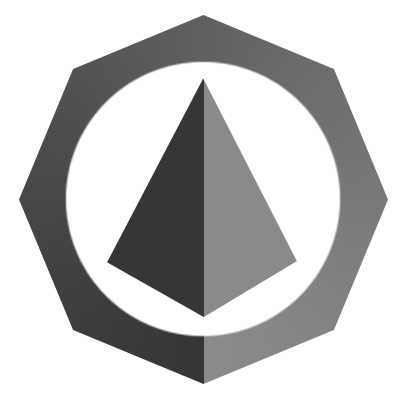
\includegraphics[width=0.15\textwidth]{Graphs/logo3.jpg}\\[0.6cm]
\textsc{\huge DAB}\\[1cm]

%Title
\HRule \\[0.75cm]
{ \huge \bfseries Decentralized Autonomous Bank}\\[0.4cm]
\HRule \\[1.5cm]
\textsc{\LARGE WHITEPAPER}\\[0.5cm]

\vfill
% Bottom of the page
{\large Final Version: \today}

\end{center}
\end{titlepage}

\section{Introduction}
A bank is a financial institution that pools social wealth and resources to make events. In a way, the banking system helps promote economic prosperity and assures assets safety: loaning starting capitals for start-ups and entrepreneurs, and at the same time generating interest for depositors. However, traditional structures and modes of economy have been changing with the advent of new technologies, like Blockchain and Smart Contracts. In recent years, people have gradually got accustomed to various types of virtual currencies and applications based on them, which have not got a sound and reliable platform like a bank to invest and earn profits yet. Thus, a call for banking systems of virtual currencies arises.
On one hand, traditional banks hold a large share of the profits, which should have belonged to both depositors and loanees. Besides, people are not contented with this hierarchical administration because of its low efficiency and manifold restrictions. The procedures of loaning include numerous risks assessment and audit work. These complicated and repetitive operations increase unnecessary costs both in labor and in material, adding to inconvenience of a loan.
Therefore, we propose a self-governed banking system transplanted on Blockchain, naming \textbf{Decentralized Autonomous Bank}, \textbf{DAB} for short. 
This will be \underline{the first} crowdfunded Ethereum banking system on Blockchain in history. The main contributions of this program are as follows:

\begin{itemize}
   \item The proposed banking system is \textbf{crowdfunded} by common users rather than authorities. With Blockchain technology, data of transactions generated by users can be recorded more accurately, and meanwhile these records can neither be modified nor be tracked by anyone, assuring its reliability and security.
   \item The proposed banking system transforms the abstract concept, ``credit,'' into measurable units for new asset class of ``\textbf{tokens}'' that are typically produced through smart contracts to cut out unnecessary procedures for assessment and approval.
   \item As the first \textbf{Ethereum bank} on Blockchain, users of which can enjoy relatively high interest when depositing their Ethereum in the bank and cheaper yet more convenient loaning services than one can do in actual banks.
\end{itemize}

The rest of this paper is structured as follows. Section 2 gives a detailed instruction of DAB. How the banking system will be crowdfunded, established and officially get down to functioning is presented in Section 3. Based on the system, section 4 describes DAB's expected outcome in the market of Ethereum. Section 5 refers to recent work and our progress on DAB. Section 6 provides a list of terminologies concerned in the paper.

\section{Concepts and Functions}
As mentioned above, not only users can deposit, withdraw, lend, loan or repay Ethereum more cost-effective in this crowdfunded DAB, but also procedures on risks assessment and credit approval are simplified. To realize these regular functions, we establish a DAB hierarchy, where users themselves can modify and improve this banking system at \textbf{DAO} (\textbf{ Distributed Autonomous Organization}) level, and enjoy services mentioned above at DAB level. There are three main departments in charge of depositing issues, loaning issues and user operations. A group of related new concepts will be introduced below, which contains four types of tokens, two sub-banks, two main contracts, \emph{etc}.

\begin{figure}[H]
\begin{center}
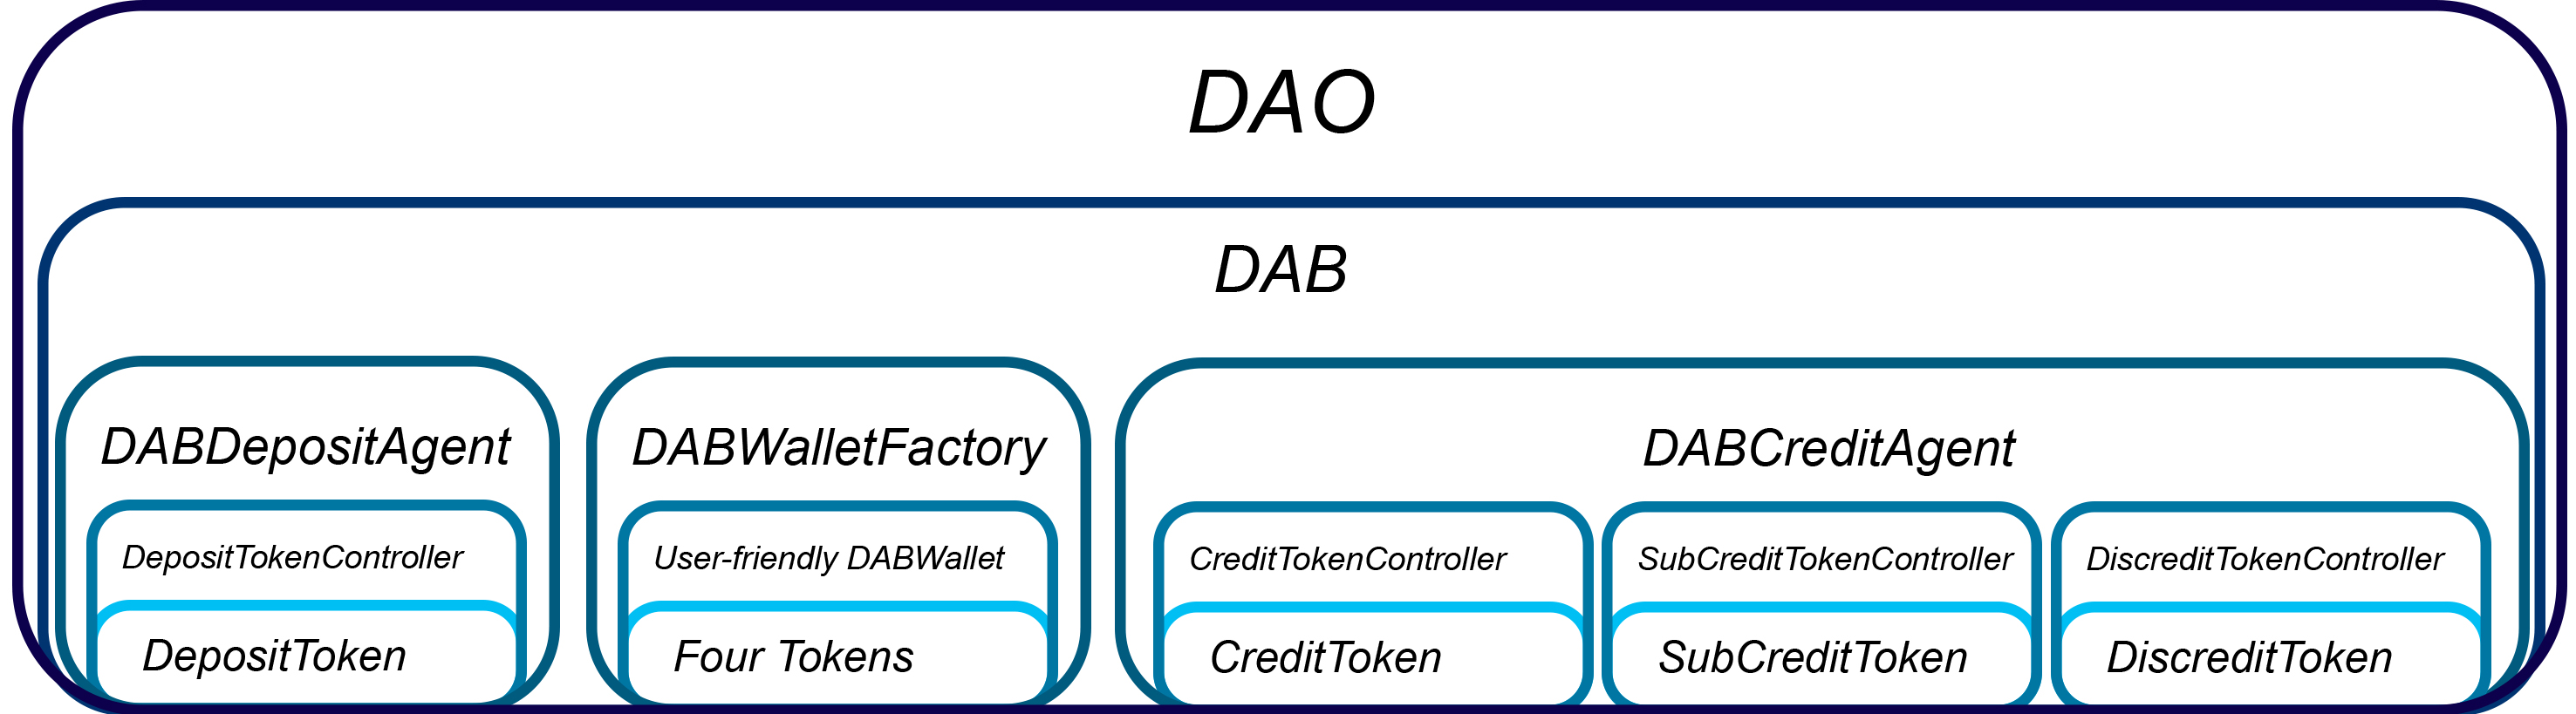
\includegraphics[width=4.5in]{Graphs/DAB_Hierarchy.jpg}
\end{center}
\caption{Hierarchy of DAB}\label{HoD}
\end{figure}

\subsection{Tokens}
\textbf{Deposit Token} (\textbf{DPT} for short) is a type of token for depositing function, while \textbf{CreditToken} (\textbf{CDT} for short) and \textbf{Sub-Credit Token} (\textbf{SCT} for short) are collectively referred to for loaning function under a joint name, \textbf{Generalized Credit Token}. As to \textbf{Discredit Token} (\textbf{DCT} for short), it is a type of token indicating one's loss of credit.

\begin{figure}[H]
\begin{center}
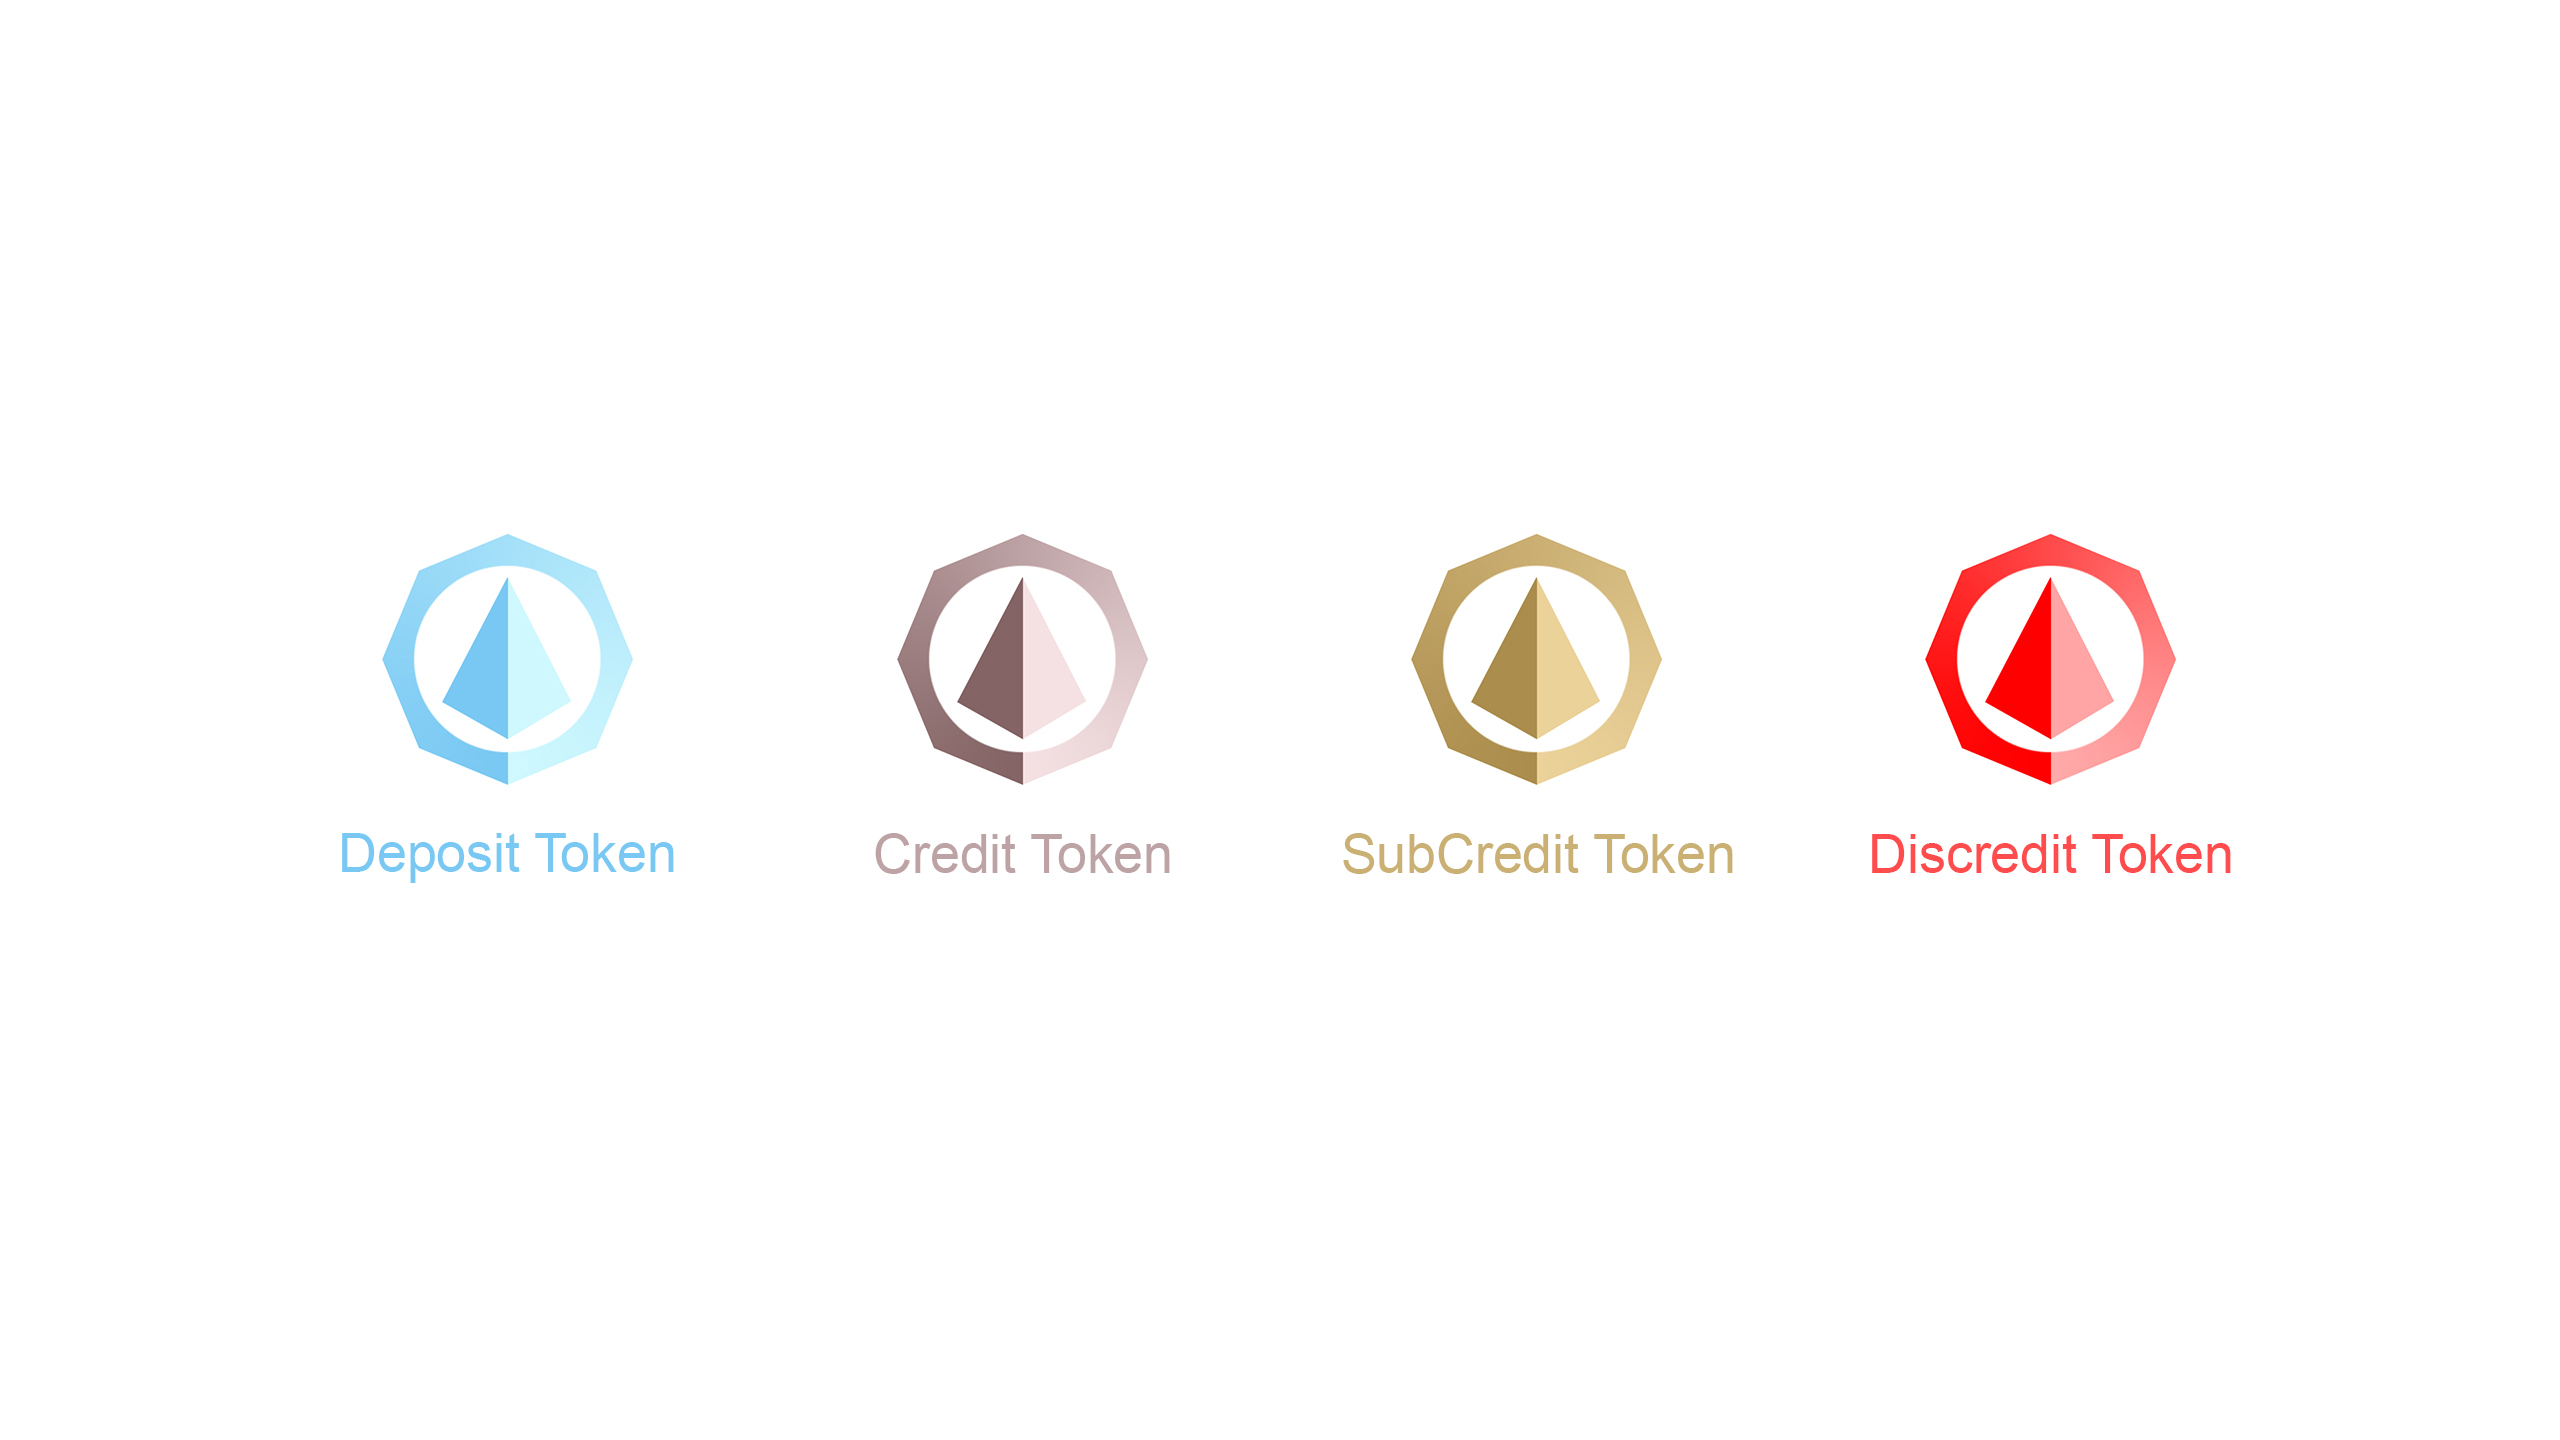
\includegraphics[width=4.5in]{Graphs/logos-line.jpg}
\end{center}
\caption{Four Tokens}\label{FT}
\end{figure}

\begin{itemize} 
   \item \textbf{Deposit Token (DPT)}: a type of token for a certain amount of Ethereum that is deposited into the bank. Each token represents a share one holds in the pool of \textbf{Deposit Reserve Fund}. DPT is negotiable in the market and can be either transferred or withdrawn.
   \item \textbf{Credit Token (CDT)}: a type of token for a certain amount of Ethereum that one user can loan from the bank. Each token represents a share one holds in the pool of \textbf{Credit Reserve Fund} aa well as the user's credit ceiling. CDT is negotiable in the market and can be cashed from Credit Bank with 10\% fees.
   \item \textbf{Sub-Credit Token (SCT)}: the secondary form of CDT in the process of a loan, which represents a condition in debt. If the loan is repaid in time, SCT will be elevated back to CDT; if not, the SCT will be converted to DCT, whose value is far less than that of CDT. SCT is an non-negotiable token in the market, with less value than that of CDT, and can be neither transferred nor cashed.
   \item \textbf{Discredit Token (DCT)}: a type of token converted from DCT if a user's debt is overdue, which indicates one's bad credit. It is of less value than SCT. The conversion from SCT to DCT is accompanied by 20\% irreversible loss, but the remnants can be converted back to CDT once the debt is paid off anytime. Although DCT cannot be cashed, it can be transferred to another user, if the user is willing to discharge the loanee's debt.
\end{itemize}

\subsection{Sub-Banks}
DAB is comprised of two independent sub-banks, which are Deposit Bank and Credit Bank. For each bank, there is a pool of reserve fund in it.
\begin{itemize} 
   \item \textbf{Deposit Bank}: a sub-bank where in most cases users deposit Ethereum getting DPT as token, gain deposit interest, and withdraw their Ethereum with the tokens. The sum of Ethereum and Deposit Tokens deposited is called a pool of \textbf{Deposit Reserve Fund}. Operations on the Deposit Bank are regulated by \textbf{Deposit Contract}.
   \item \textbf{Credit Bank}: a sub-bank where in most cases users loan and repay Ethereum, and gain bonus CDT as reward. The sum of Ethereum and Credit Tokens in this sub-bank is called a pool of \textbf{Credit Reserve Fund}. Operations on the Credit Bank are regulated by \textbf{Credit Contract}.
\end{itemize}

\subsection{Contracts}
The two main contracts are \textbf{Deposit Contract} and \textbf{Credit Contract}, which are responsible for the bank's depositing function and loaning function, respectively.

\begin{itemize} 
   \item \textbf{Deposit Contract}: a protocol with which deposit-related operations occur and Deposit Bank runs in accordance, such as users depositing Ethereum into Deposit Bank, withdrawing Ethereum with DPT, transferring DPT to other users, \emph{etc}. The contract also stipulates that \textbf{Deposit Cash Reserve Ratio} is automatically adjusted with the variation of negotiable Deposit Tokens in the market, thereby calculating a withdrawal price of a DPT at a certain point.
   \item \textbf{Credit Contract}: a protocol with which credit-related operations occur and Credit Bank runs in accordance, such as users loaning Ethereum from Credit Bank with CDT, repaying Ethereum, cashing CDT, gaining bonus CDT, CDT degrading, DCT transferring and conversion, \emph{etc}. The contract also stipulates that the cashed price of a CDT is dependent on the amount of \textbf{Credit Reserve Fund}, \textbf{Credit Cash Reserve Ratio} and the number of negotiable Credit Tokens in the market, altogether.
\end{itemize}

\subsection{A Wallet}
\textbf{DAB Wallet} is a user-oriented wrapper in charge of deposit-related and credit-related operations. As a wrapper of DAB, users can accomplish inquiring, depositing, loaning, transferring, cashing and other operations much more conveniently with fewer procedures. With regards to \textbf{DAB Wallet}, it works as a set of interfaces of these various operations, which minimize the incidence of mistakes.

\subsection{An Organization}
\textbf{Distributed Autonomous Organization, DAO for short} is the decision-making level of DAB. Each user has the right to put forward proposals onto the pending list in DAO, whose issues may concern interest adjustments, mintage suppression and so on. Users vote on these proposals to improve the mechanism and adaptability of DAB in virtual currency market. The weight of a vote directly relies on the number of Deposit Tokens one has.

\subsection{Behaviors}
This sub-section focuses on what users can do in DAB. The main five behaviors that users may carry out are listed below.

\begin{itemize}
   \item Fund and purchase. Before DAB begins to function officially, every single person who funds it is regarded as a founder and a user of it, and a certain proportion of the funds acts as purchase of DPT and reward of CDT in return. This is the primary way to gain tokens in DAB.
   \item Deposit and withdraw. After DAB's official running, for one thing, a user can deposit Ethereum into Deposit Bank, get equivalent Deposit Tokens for a certain share of \textbf{Deposit Reserve Fund}, and enjoy interest from it. This is another way to gain Deposit Tokens in DAB. For another, user can withdraw Ethereum and return his/her Deposit Tokens back to the bank.
   \item Loan and repay. After DAB's official running, a user can loan Ethereum from Credit Bank according to the number of Credit Tokens he/she owns. Once he/she prepays a certain amount of interest according to his/her loaning plan, he/she will receive the loan of Ethereum and equivalent Credit Tokens are degraded to Sub-Credit Tokens immediately. A certain percentage of the prepaid interest will be used for producing new Credit Tokens dependent on \textbf{Deposit Cash Reserve Ratio}, \textbf{CRR(DPT)} or \textbf{CRR} for short, and then those will be rewarded to the user. The completion of the loan will trigger a conversion from Sub-Credit Tokens to Credit Tokens equivalent in their number. This is another way to gain Credit Tokens in DAB. But Sub-Credit Tokens will be converted to Discredit Tokens with 20\% loss if the debt is not returned timely. The ownership of DCT indicates bad credit of the user.
   \item Transfer. Most forms of assets can be transferred between users, including Ethereum, DPT, CDT and DCT (not SCT). Especially, the transfer of DCT is another solution for a user discharging his/her debt, if he is willing to. But risks of this operation over-ranges DAB's responsibility.
   \item Cash CDT. Commonly, after DAB's official running, CDT serves as a measure of one's credit ceiling, \emph{i.e.} the maximum Ethereum one can loan from DAB. Despite that the cashed price of each CDT is lower than its credit line, CDT can still be one-way cashed to Ethereum, if needed.
\end{itemize}

\section{Implementation}
DAB is a crowdfunding project, so its final foundation and implementation cannot be realized without funds from public. Therefore, this project warmly welcomes those who have belief in DAB or are willing to give it a try to provide Ethereum support to the bank. 
In this crowdfunding phase, there are three primary jobs: people investing Ethereum to fund DAB, DAB minting tokens, and tokens being allocated to users (DPT as a share of deposit and CDT as a measure of credit). Along with the jobs progress, \textbf{Deposit Contract} and \textbf{Credit Contract} are successively activated, which is referred to as \textbf{Activation Stage}. After the activation of \textbf{Credit Contract}, \textbf{Expansion Stage} begins, indicating DAB's official on-line running.

\subsection{Activation Stage}
In Activation Stage, people deposit Ethereum into DAB, and then Deposit Tokens and Credit Tokens are proportionally produced to be allocated to the funders in return. Before the activation of \textbf{Deposit Contract}, users can not withdraw DPT, while CDT can neither be cashed nor be used for loaning Ethereum before the activation of \textbf{Credit Contract}. But transferring is permitted all the time.

\begin{figure}[H]
\begin{center}
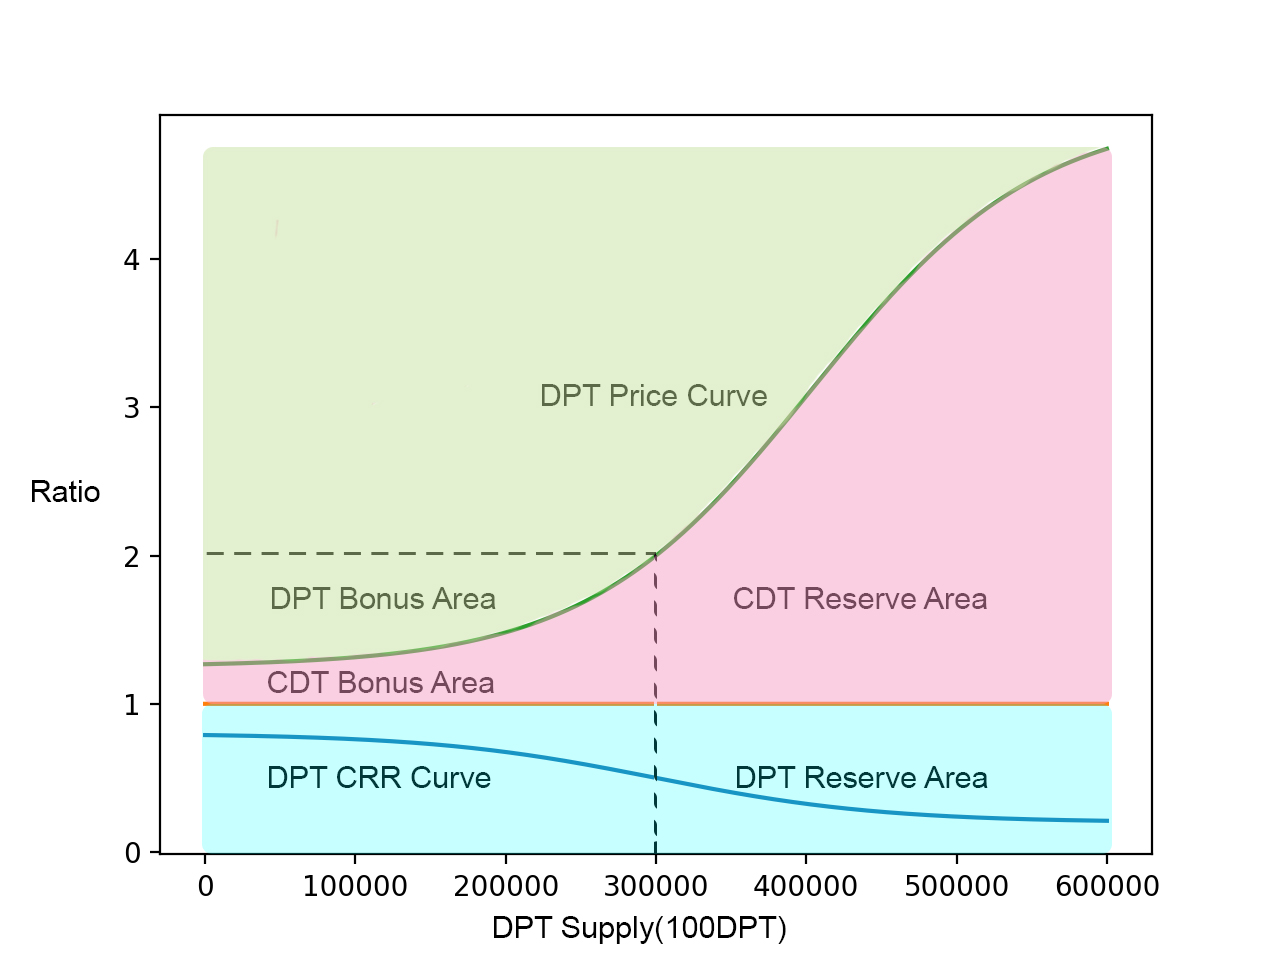
\includegraphics[width=4.5in]{Graphs/Activation1.jpg}
\end{center}
\caption{Activation Stage}\label{AS}
\end{figure}

The exact proportion of Deposit Tokens and Credit Tokens produced per Ethereum is directly dependent on \textbf{CRR}. Each Ethereum funded is for producing Deposit Tokens and a reward of \emph{(1 - CRR)} is for producing Credit Tokens. Former funders get more Deposit Tokens per Ethereum than Credit Tokens because DPT is cheaper in the earlier stage. But as the mintage of Deposit Tokens proceeds, shown as the blue curve \textbf{DPT CRR Curve} in Fig. \ref{AS}, \textbf{CRR} drops with the number of produced tokens rising, thereby rendering latter users to get more Credit Tokens per Ethereum than Deposit Tokens. The orange curve stands for situations when \textbf{CRR} is a constant of $1$, and what is below is \textbf{DPT Reserve Area}, representing \textbf{Deposit Reserve Fund}. Note that the number of produced Deposit Tokens is equivalent to that of negotiable ones before activation, for they cannot be withdrawn yet.
As regards to issuance price of the two tokens, DPT's starts with ${\frac{1}{100}}$ Ethereum per token while CDT's is a constant of ${\frac{1}{50}}$. As Fig. \ref{AS} is shown, the green curve represents the functional relationship between the issuance price of DPT and its produced number, which has an increasing trend. What is above the green curve is \textbf{DPT Bonus Area}, while what is between the orange and green curve is \textbf{CDT Reserve Area}, which represents \textbf{Credit Reserve Fund}. Because all the Credit Tokens acquired is a reward from depositing, \textbf{CDT Reserve Area} is equivalent to \textbf{CDT Bonus Area}  as well. Consequently, former funders purchase DPT at a lower price which is of higher value.
Nevertheless, this does not mean that latter funders fail to get a good bargain, for they get more Credit Tokens than the former ones get, indicating higher amount of ``credit.'' Such mechanism is set to assure all the funders, former or latter, can benefit from DAB in whatever ways.
\textbf{Deposit Contract} will be activated once the two-week-long projected activation time is up. The activation of \textbf{Deposit Contract} will then be followed by a two-week-long activation of \textbf{Credit Contract}, which is due at the end of the second week after.

\subsection{Expansion Stage}
The activations are market-driven, which is much self-adaptive and more robust than any other existing ICOs. Besides, before the activations, neither the token transferring behavior is restricted, nor the profits for those developers and maintainers are dear for users to take, which making it much cheaper and more funder-friendly.
After the activation of \textbf{Deposit Contract}, users are able to withdraw DPT. What's more, users can cash CDT and use CDT for loaning Ethereum after the activation of \textbf{Credit Contract}. From this point, basically all the functions of DAB are open to public.

\begin{figure}[H]
\begin{center}
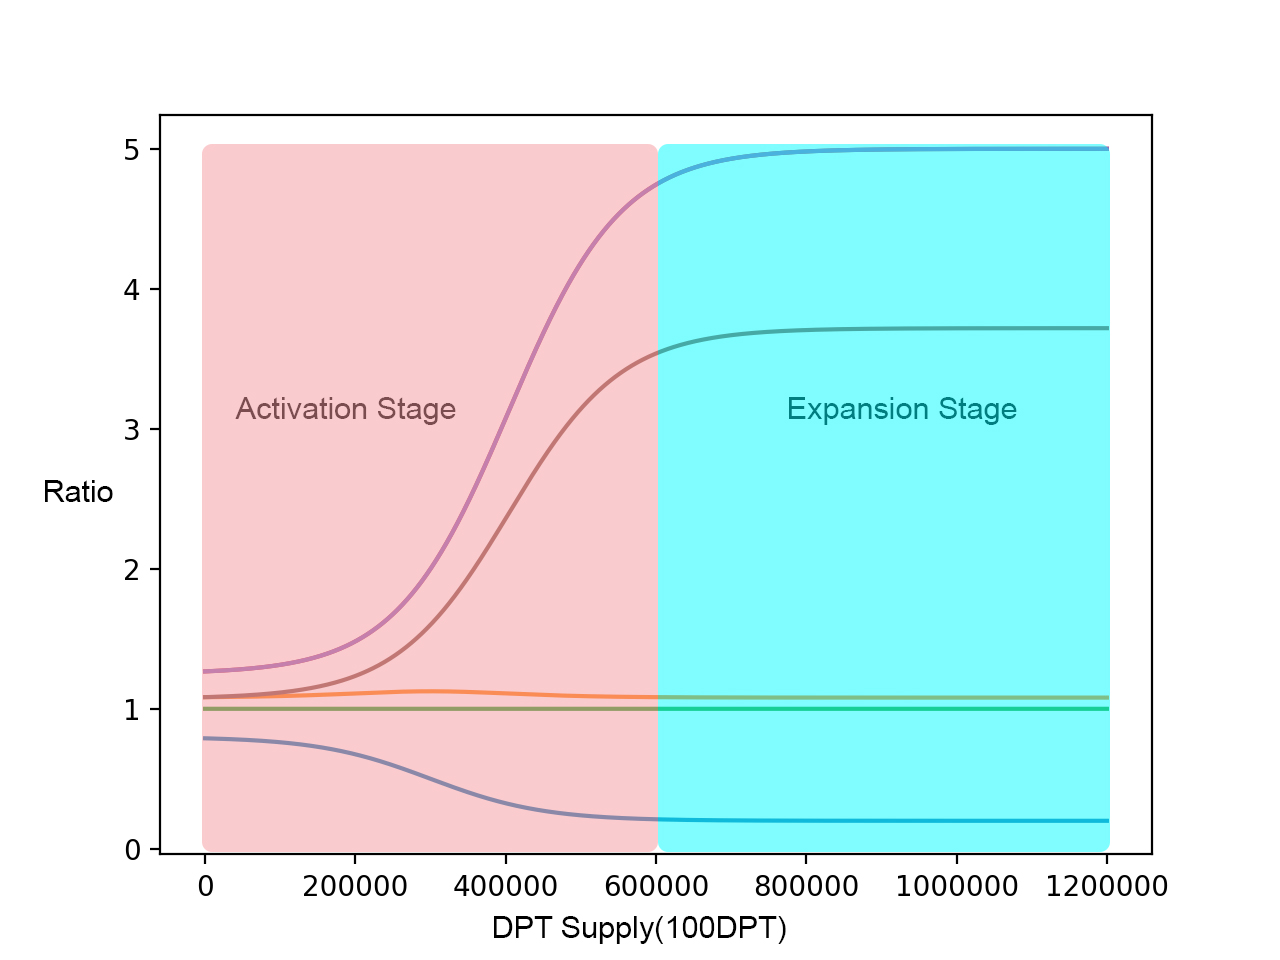
\includegraphics[width=4.5in]{Graphs/Two_Stage.jpg}
\end{center}
\caption{Two Stage}\label{TS}
\end{figure}

To assure a stable market, a certain percentage of the funds will serve as profits for mintage to those who develops and maintains DAB. As the mintage proceeds, DPT becomes more expensive. To suppress excessive production of DPT, the profits for mintage increases as the rise of DPT's price. Besides, users are encouraged to loan, for they can acquire more Credit Tokens, driving the price of DPT stick to \textbf{DPT Price Curve}. As Fig. \ref{TS} illustrates, with more and more people depositing and loaning, the produced number of tokens increases until their price and reserve ratio are approximately stabilized, which is referred to as Expansion Stage. The brown curve in Fig. \ref{TS} represents the revenue of the first funder, while the orange curve represents the revenue of a funder at any time. Expansion Stage, the bank grows robust and adaptive enough to resist and react timely with the uncertain market automatically.

\begin{figure}[H]
\begin{center}
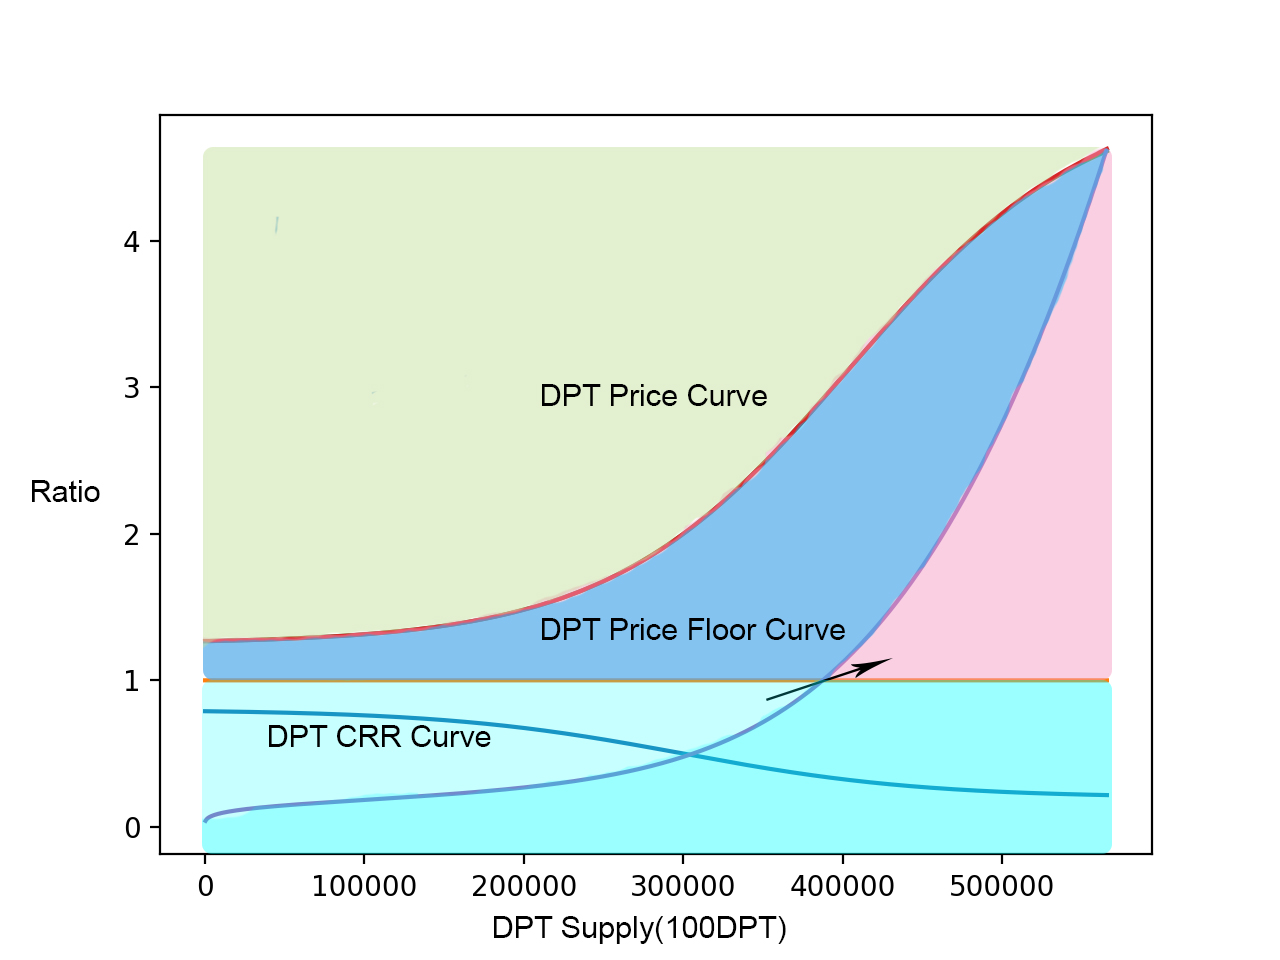
\includegraphics[width=4.5in]{Graphs/PriceFloorCurve.jpg}
\end{center}
\caption{Price Floor Curve}\label{PFC}
\end{figure}

DAB in Expansion Stage functions stably, not inclined to be maliciously manipulated. Also, the blue \textbf{Price Floor Curve} in Fig. \ref{PFC} shows that with negotiable Deposit Tokens shrinking, the ratio of DPT's value over its price rises drastically to hold back the price's trend to drop.

\subsection{Incentives for Token Holders}
Different incentives are employed by DAB to encourage users to either deposit or loan. Fig. \ref{II} vividly illustrates the interactions among Deposit Bank, Credit Bank and a user \emph{Aaron}, which helps understand DAB's functioning mechanism better.

\begin{figure}[H]
\begin{center}
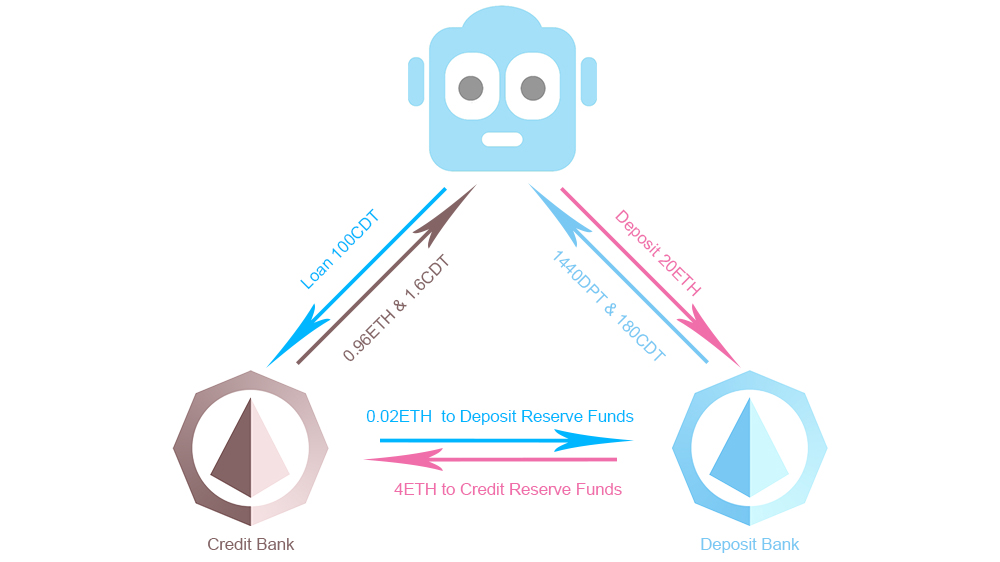
\includegraphics[width=4.5in]{Graphs/InterestDistribution.jpg}
\end{center}
\caption{Incentives Interactions}\label{II}
\end{figure}

Take this picture for an example, where ${CRR = 80\%}$, ${Price(DPT) = 0.01/CRR = 0.0125}$, ${Price(CDT) = 0.02}$, the maximum amount of Ethereum one can loan per CDT ${Loan(CDT) = 0.01}$ and ${Interest(Loan) = 4\%}$. When \emph{Aaron} wants to deposit $20$ Ethereum into Deposit Bank, ${\frac{1 - CRR}{2} = 10\%}$ of the deposit serves as profits for developers and maintainers, for whom those will be used to produce tokens, while the rest ${1 - \frac{1 - CRR}{2} = \frac{1 + CRR}{2} = 90\%}$ will be used to produce tokens for users. All the deposit will be spent on producing ${\frac{20 \* \frac{(1 + CRR)}{2}}{Price(DPT)} = 1440}$ Deposit Tokens, which represent the users' share held in Deposit Bank. And a $20\%$ reward (of $4$-Ethereum value) will be used for producing ${\frac{20 \* (1 - CRR) \* \frac{1 + CRR}{2}}{Price(CDT)} = 180}$ Credit Tokens, which serves as incentives for his/her depositing behavior. If \emph{Aaron} wants to apply for a loan using 100 Credit Tokens, he has to freeze them first as Sub-Credit Tokens, and then receive ${100 \* Loan(CDT) \* (1 - Interest(Loan)) = 0.96}$ Ethereum, which has already subtracted the prepaid interest and corresponding bonus ${\frac{100 \* Loan(CDT) \* Interest(Loan) \* CRR}{Price(CDT)} = 1.6}$ CDT as incentives. Also, half of the interest, whose value is of 0.02 Ethereum, will be transited to \textbf{Deposit Reserve Fund} in Deposit Bank as the interest for those depositors.
The incentives for a loan and a deposit varies in condition of different \textbf{CRR} and prices. For instance, when the frequency of depositing behavior far outnumbers that of loaning behavior, the incentives for depositing fall and those for loaning rise to encourage users to loan otherwise.

\section{Expectations}
What Distributed Autonomous Bank attempts to achieve is to establish a harmonious ecosystem for basic monetary behaviors on Ethereum. This autonomous bank can function well in most cases without any administration or supervision from authorities. Normally, without much maintenance, the pre-designed mechanism can accomplish variations and adjustments of indices like tokens' price and deposit's interest. For the reason that labors and time are saved, users in DAB enjoys higher interest when depositing and lower one when loaning.
There are three core functions in this ecosystem, which are funding, crediting and profiting. People fund the bank become its users, being given a certain amount of credit to, and the funds can provide adequate Ethereum for users in need. The users who enjoys cheaper loans hand in interest to the bank, some of which is re-allocated to depositors (funders) as anti-inflation reserve. This reserve part reduces the risk of users' investment. At the same time, honest behaviors will be further rewarded by raising the users' credit ceiling by bonus CDTs. What's more, the abstract concept of ``credit'' now becomes a measurable unit of currency that can be transacted in the market of DAB, adding convenience and reducing risks of the whole system. The three functions are bonded with and meanwhile promoted by one another, thus rendering a healthy ecosystem.

\section{Recent Work}

We have already completed the code base for the alpha test, though it is not open-sourced yet. The open-sourced ABI of DAB contracts have been posted on \textbf{Github}: \underline{https://github.com/dabdevelop/ABI}. And more details can be found on our \textbf{Wiki}: \underline{https://dab.wiki/}. Please feel free to follow us via other social networking platforms.

\begin{itemize}
   \item \textbf{Facebook}: \underline{https://www.facebook.com/DecentralizedAutonomousBank}
   \item \textbf{Twitter}: \underline{https://twitter.com/dab\_foundation}
   \item \textbf{Youtube}: \underline{https://www.youtube.com/channel/UCZpjr9qlsY-NZ2yDUy3A5Og}
   \item \textbf{Medium}: \underline{https://blog.dab-foundation.org}
   \item \textbf{Slack}: \underline{https://dab-foundation.slack.com}
\end{itemize}

\section{Important Notice}
Please read this section very carefully, and it is highly recommended that you should consult your legal, financial, tax or other professional advisor(s) if you have any doubts in the action you may take.
The DAB team is not intended to constitute securities in any jurisdiction. This Whitepaper does not constitute a prospectus or offer document of any sort and is not intended to constitute an offer of securities or a solicitation for investment in securities in any jurisdiction. 
This Whitepaper does not constitute or form part of any opinion on any advice to sell, or any solicitation of any offer by developers of DAB to purchase any types of the four tokens nor shall it or any part of it nor the fact of its presentation form the basis of, or be relied upon in connection with, any contracts or investment decision. 
The developers will be an affiliate of DAB. Ltd., and will deploy all proceeds of production of the four types of tokens to fund DAB's cryptocurrency project, businesses and operations. 
No person is bound to enter into any literal contracts or binding legal commitment in relation to the transaction and purchase of any types of the four tokens and no cryptocurrency or other form of payment is to be accepted on the basis of this Whitepaper. 
Any agreement as between DAB and you as a user or a funder, and in relation to any transaction and purchase, of the four tokens (as referred to in this Whitepaper) is to be governed by only a separate document setting out the terms and conditions (the ``T\&Cs'') of such agreement. In the event of any inconsistencies between the T\&Cs and this Whitepaper, the former shall prevail.
No regulatory authority has examined or approved of any of the information set out in this Whitepaper. No such action has been or will be taken under the laws, regulatory requirements or rules of any jurisdiction. The publication, distribution or dissemination of this Whitepaper does not imply that the applicable laws, regulatory requirements or rules have been complied with. 
There are risks and uncertainties associated with DAB and/or the developer and their respective businesses and operations, any types of the four tokens, the activation of \textbf{Deposit Contract} and \textbf{Credit Contract} and the DAB Wallet (each as referred to in this Whitepaper). 
This Whitepaper, any part thereof and any copy thereof must not be taken or transmitted to any country where distribution or dissemination of this Whitepaper is prohibited or restricted. 
No part of this Whitepaper is to be reproduced, distributed or disseminated without including this section.

\subsection{Disclaimer of Liability}
To the maximum extent permitted by the applicable laws, regulations and rules, DAB or its developers shall not be liable for any indirect, special, incidental, consequential or other losses of any kind, in tort, contract or otherwise (including but not limited to loss of revenue, income or profits, and loss of use or data), arising out of or in connection with any acceptance of or reliance on this Whitepaper or any part thereof by you. 

\subsection{No Representations and Warranties}
DAB or its developers do not make or purport to make, and hereby disclaims, any representation, warranty or undertaking in any form whatsoever to any entity or person, including any representation, warranty or undertaking in relation to the truth, accuracy and completeness of any of the information set out in this Whitepaper. 

\subsection{Representations and Warranties by You}
By accessing and/or accepting possession of any information in this Whitepaper or such part thereof (as the case may be), you represent and warrant to DAB or its developers as follows: 

\begin{enumerate}
   \item you agree and acknowledge that DAB's four types of tokens do not constitute securities in any form in any jurisdiction;
   \item you agree and acknowledge that this Whitepaper does not constitute a prospectus or offer document of any sort and is not intended to constitute an offer of securities in any jurisdiction or a solicitation for investment in securities and you are not bound to enter into any contracts or binding legal commitment and no cryptocurrency or other form of payment is to be accepted on the basis of this Whitepaper;
   \item you agree and acknowledge that no regulatory authority has examined or approved of the information set out in this Whitepaper, no action has been or will be taken under the laws, regulatory requirements or rules of any jurisdiction and the publication, distribution or dissemination of this Whitepaper to you does not imply that the applicable laws, regulatory requirements or rules have been complied with;
   \item you agree and acknowledge that this Whitepaper, the undertaking and/or the completion of the activation of \textbf{Deposit Contract} and \textbf{Credit Contract}, or future trading in DAB on any cryptocurrency exchange, shall not be construed, interpreted or deemed by you as an indication of the merits of the DAB or its developers, any types of the four tokens, the activation of two contracts and DAB Wallet (each as referred to in this Whitepaper);
   \item the distribution or dissemination of this Whitepaper, any part thereof or any copy thereof, or acceptance of the same by you, is not prohibited or restricted by the applicable laws, regulations or rules in your jurisdiction, and where any restrictions in relation to possession are applicable, you have observed and complied with all such restrictions at your own expense and without liability to DAB and/or its developers;
   \item you agree and acknowledge that in the case where you wish to purchase any types of the four tokens, the tokens are not to be construed, interpreted, classified or treated as:
\begin{itemize}
   \item any kind of currency other than cryptocurrency;
   \item debentures, stocks or shares issued by any person or entity in DAB.
   \item rights, options or derivatives in respect of such debentures, stocks or shares;
   \item units in a collective investment scheme;
   \item units in a business trust;
   \item derivatives of units in a business trust;
   \item or any other security or class of securities.
\end{itemize}

   \item you have a basic degree of understanding of the operation, functionality, usage, storage, transmission mechanisms and other material characteristics of cryptocurrencies, blockchain-based software systems, cryptocurrency wallets or other related token storage mechanisms, blockchain technology and smart contract technology;
   \item you are fully aware and understand that in the case where you wish to fund DAB, there are risks associated with DAB and its respective business and operations, any types of the four tokens, the activation of the two contracts and the DAB Wallet (each as referred to in the Whitepaper);
   \item you agree and acknowledge that neither DAB nor its developers is liable for any indirect, special, incidental, consequential or other losses of any kind, in tort, contract or otherwise (including but not limited to loss of revenue, income or profits, and loss of use or data), arising out of or in connection with any acceptance of or reliance on this Whitepaper or any part thereof by you; and rights under a contract for differences or under any other contracts the purpose or pretended purpose of which is to secure a profit or avoid a loss;
   \item all of the above representations and warranties are true, complete, accurate and non-misleading from the time of your access to and/or acceptance of possession this Whitepaper or such part thereof (as the case may be).
\end{enumerate}

\subsection{Cautionary Note on Forward-looking Statements}
All statements contained in this Whitepaper, statements made in press releases or in any place accessible by the public and oral statements that may be made by DAB and/or its developers or their respective directors, executive officers or employees acting on behalf of DAB or its developers (as the case may be), that are not statements of historical fact, constitute ``forward-looking statements.'' Some of these statements can be identified by forward-looking terms such as ``aim,'' ``target,'' ``anticipate,'' ``believe,'' ``could,'' ``estimate,'' ``expect,'' ``if,'' ``intend,'' ``may,'' ``plan,'' ``possible,'' ``probable,'' ``project,'' ``should,'' ``would,'' ``will'' or other similar terms. However, these terms are not the exclusive means of identifying forward-looking statements. All statements regarding DAB's and/or its developers' financial position, business strategies, plans and prospects and the future prospects of the industry which DAB and/or its developers is in are forward-looking statements. These forward-looking statements, including but not limited to statements as to DAB's and/or its developers' revenue and profitability, prospects, future plans, other expected industry trends and other matters discussed in this Whitepaper regarding DAB and/or its developers are matters that are not historic facts, but only predictions. 
These forward-looking statements involve known and unknown risks, uncertainties and other factors that may cause the actual future results, performance or achievements of DAB and/or its developers to be materially different from any future results, performance or achievements expected, expressed or implied by such forward-looking statements. These factors include, amongst others: 

\begin{itemize}
   \item changes in political, social, economic and stock or cryptocurrency market conditions, and the regulatory environment in the countries in which DAB and/or its developers conducts its respective businesses and operations;
   \item the risk that DAB and/or its developers may be unable or execute or implement their respective business strategies and future plans;
   \item changes in interest rates and exchange rates of fiat currencies and cryptocurrencies;
   \item changes in the anticipated growth strategies and expected internal growth of DAB and/or its developers;
   \item changes in the availability and fees payable to DAB and/or its developers in connection with their respective businesses and operations;
   \item changes in the availability and salaries of employees who are required by DAB and/or its developers to operate their respective businesses and operations;
   \item changes in preferences of customers of DAB and/or its developers;
	\item changes in competitive conditions under which DAB and/or its developers operate, and the ability of DAB and/or its developers to compete under such conditions;
   \item changes in the future capital needs of DAB and/or its developers and the availability of financing and capital to fund such needs;
   \item war or acts of international or domestic terrorism;
   \item occurrences of catastrophic events, natural disasters and acts of God that affect the businesses and/or operations of DAB and/or its developers;
   \item other factors beyond the control of DAB and/or its developers;
   \item and any risk and uncertainties associated with DAB and/or its developers and their businesses and operations, any types of the four tokens, the activation of the two contracts and the DAB Wallet (each as referred to in the Whitepaper).
\end{itemize}

All forward-looking statements made by or attributable to DAB and/or its developers or persons acting on behalf of DAB and/or its developers are expressly qualified in their entirety by such factors. Given that risks and uncertainties that may cause the actual future results, performance or achievements of DAB and/or its developers to be materially different from that expected, expressed or implied by the forward-looking statements in this Whitepaper, undue reliance must not be placed on these statements. These forward-looking statements are applicable only as of the date of this Whitepaper. 
Neither DAB, its developers nor any other person represents, warrants and/or undertakes that the actual future results, performance or achievements of DAB and/or its developers will be as discussed in those forward-looking statements. The actual results, performance or achievements of DAB and/or its developers may differ materially from those anticipated in these forward- looking statements. 
Nothing contained in this Whitepaper is or may be relied upon as a promise, representation or undertaking as to the future performance or policies of DAB and/or its developers. 
Further, DAB and/or its developers disclaim any responsibility to update any of those forward- looking statements or publicly announce any revisions to those forward-looking statements to reflect future developments, events or circumstances, even if new information becomes available or other events occur in the future. 

\subsection{Market and Industry Information and No Consent of Other Persons}
This Whitepaper includes reports and studies, where appropriate, as well as market research, publicly available information and industry publications. Such surveys, reports, studies, market research, publicly available information and publications generally state that the information that they contain has been obtained from sources believed to be reliable, but there can be no assurance as to the accuracy or completeness of such included information. 
Save for DAB, its developers and their respective directors, executive officers and employees, no person has provided his or her consent to the inclusion of his or her name and/or other information attributed or perceived to be attributed to such person in connection therewith in this Whitepaper and no representation, warranty or undertaking is or purported to be provided as to the accuracy or completeness of such information by such person and such persons shall not be obliged to provide any updates on the same. 
While DAB and/or its developers have taken reasonable actions to ensure that the information is extracted accurately and in its proper context, DAB and/or its developers have not conducted any independent review of the information extracted from third party sources, verified the accuracy or completeness of such information or ascertained the underlying economic assumptions relied upon therein. Consequently, neither DAB, its developers, nor their respective directors, executive officers and employees acting on their behalf makes any representation or warranty as to the accuracy or completeness of such information and shall not be obliged to provide any updates on the same. 

\subsection{Terms Used}
To facilitate a better understanding of any types of the four tokens being offered for purchase by its developers, and the businesses and operations of DAB and/or its developers, certain technical terms and abbreviations, as well as, in certain instances, their descriptions, have been used in this Whitepaper. These descriptions and assigned meanings should not be treated as being definitive of their meanings and may not correspond to standard industry meanings or usage. 
Words importing the singular shall, where applicable, include the plural and vice versa and words importing the masculine gender shall, where applicable, include the feminine and neuter genders and vice versa. References to persons shall include corporations. 

\subsection{No Advice}
No information in this Whitepaper should be considered to be business, legal, financial or tax advice regarding DAB, its developers, any types of the four tokens, the activation of the two contracts and the DAB Wallet (each as referred to in the Whitepaper). You should consult your own legal, financial, tax or other professional adviser regarding DAB and/or its developers and their respective businesses and operations, any types of the four tokens, the activation of the two contracts and the DAB Wallet (each as referred to in the Whitepaper). You should be aware that you may be required to bear the financial risk of any purchase of any types of the four tokens for an indefinite period of time. 

\subsection{No Further Information or Update}
No person has been or is authorized to give any information or representation not contained in this Whitepaper in connection with DAB and/or its developers and their respective businesses and operations, any types of the four tokens, the activation of the two contracts and the DAB Wallet (each as referred to in the Whitepaper) and, if given, such information or representation must not be relied upon as having been authorized by or on behalf of DAB and/or its developers. The activation of the two contracts (as referred to in the Whitepaper) shall not, under any circumstances, constitute a continuing representation or create any suggestion or implication that there has been no change, or development reasonably likely to involve a material change in the affairs, conditions and prospects of DAB and/or its developers or in any statement of fact or information contained in this Whitepaper since the date hereof.

\subsection{Restrictions on Distribution and Dissemination}
The distribution or dissemination of this Whitepaper or any part thereof may be prohibited or restricted by the laws, regulatory requirements and rules of any jurisdiction. In the case where any restriction applies, you are to inform yourself about, and to observe, any restrictions which are applicable to your possession of this Whitepaper or such part thereof (as the case may be) at your own expense and without liability to DAB and/or its developers. 
Persons to whom a copy of this Whitepaper has been distributed or disseminated, provided access to or who otherwise have the Whitepaper in their possession shall not circulate it to any other persons, reproduce or otherwise distribute this Whitepaper or any information contained herein for any purpose whatsoever nor permit or cause the same to occur.

\subsection{No Offer of Securities or Registration}
This Whitepaper does not constitute a prospectus or offer document of any sort and is not intended to constitute an offer of securities or a solicitation for investment in securities in any jurisdiction. No person is bound to enter into any contracts or binding legal commitment and no cryptocurrency or other form of payment is to be accepted on the basis of this Whitepaper. Any agreement in relation to any transaction and purchase of any types of the four tokens (as referred to in this Whitepaper) is to be governed by only the T\&Cs of such agreement and no other document. In the event of any inconsistencies between the T\&Cs and this Whitepaper, the former shall prevail. 
You are not eligible to purchase any types of the four tokens in the activation of the two contracts (as referred to in this Whitepaper) if you are a citizen, resident (tax or otherwise) or green card holder of the United States of America or a citizen or resident of the Republic of Singapore. 
No regulatory authority has examined or approved of any of the information set out in this Whitepaper. No such action has been or will be taken under the laws, regulatory requirements or rules of any jurisdiction. The publication, distribution or dissemination of this Whitepaper does not imply that the applicable laws, regulatory requirements or rules have been complied with.

\subsection{Risks and Uncertainties}
Prospective purchasers of any types of the four tokens (as referred to in this Whitepaper) should carefully consider and evaluate all risks and uncertainties associated with DAB, its developers and their respective businesses and operations, any types of the four tokens, the activation of the two contracts and the DAB Wallet (each as referred to in the Whitepaper), all information set out in this Whitepaper and the T\&Cs prior to any purchase of any types of the four tokens. If any of such risks and uncertainties develops into actual events, the business, financial condition, results of operations and prospects of DAB and/or its developers could be materially and adversely affected. In such cases, you may lose all or part of the value of any types of the four tokens.

\end{document}